\documentclass[]{article}
\usepackage[margin = 1.3in]{geometry}

%opening
\title{Quantum Random Number Generation from Phase-induced Intensity Noise and Shot Noise}
\author{Robin Camphausen}
\date{}
%\usepackage[sorting=none]{biblatex}
%\bibliography{bibliographyFibreEye}
\usepackage{graphicx}
\usepackage{float}
\usepackage[font = {small,it}]{caption}
%\usepackage{subcaption}
\usepackage{cite}
%\bibliographystyle{unsrt}
%\usepackage{notoccite}
\usepackage{gensymb}
\usepackage{textcomp}
\usepackage{amsmath}
\usepackage{hyperref}
\usepackage{afterpage}
\usepackage[
    font={small},
    % labelfont=bf,
    % format=hang,    
    % format=plain,
    margin=0pt,
    width=0.9\textwidth,
]{caption}
\usepackage[list=true]{subcaption}
\usepackage{graphicx} %Loading the package
%\graphicspath{{../../Pictures/SPAD-QRNG/}}
\graphicspath{{./Figures/}}


\newcommand*\mean[1]{\overline{#1}}


\begin{document}
\maketitle
\section{Introduction}

	Quantum random number generators (QRNGs) are important for a large number of applications, including for finance, communication and computational modelling \cite{herrero-collantes_quantum_2017}. One way to generate quantum random numbers (QRNs) is to measure shot noise, which arises due to the quantised nature of light: when observing a light source over a given time frame a discrete number of photons will arrive at the detector and while the average number of photons stays constant there is a variance in the number of arrivals per time frame \cite{sanguinetti_quantum_2014}. It is also possible to generate QRNs by measuring phase noise, which is due to the fact that a spontaneously emitted photon has a completely random phase, uniformly distributed between $0$ and $2\pi$ \cite{xu_ultrafast_2012,abellan_ultra-fast_2014}. In this report we describe a hybrid QRNG method, which increases the randomness able to be extracted in the Shot noise method by also taking into account the random optical phases of the light source.

\section{Phase-induced Intensity Noise} 
\subsection{Theory of Intensity Noise due to Phase Fluctuations}\label{RPS}

	A single spontaneously emitted photon has random phase, but it is of course not possible to measure the phase of a single photon. In references \cite{abellan_ultra-fast_2014,mitchell_strong_2015,abellan_generation_2015} therefore, the single spontaneously emitted photon is generated inside a laser cavity, which subsequently uses stimulated emission to generate many copies of this first photon until the light intensity is large enough for an interferometric measurement of the phase. The laser must subsequently be switched off again to allow all stimulated photons in the cavity to decay, so that upon switching it on again a new spontaneously emitted photon with a new random phase can start the same process again.
	Another way of exploiting the random phase of a spontaneously emitted photon is to measure many of them at once. If all the photons are emitted such that they have statistically independent amplitudes and phases from each other, the resulting sum can be described as a Random Phasor Sum (RPS) \cite{goodman_statistical_2000}:
		\begin{equation}
		\mathbf{a} = ae^{i\theta} = \frac{1}{\sqrt{N}} \sum_{k=1}^{N} \alpha_k e^{i\phi_k}. \label{eq:RPSbasic} 
		\end{equation}
	Note that this equation is normalised. $\alpha_k /\sqrt{N}$ and $\phi_k$ are the amplitudes and phases respectively of the $K^{th}$ photon comprising the RPS. In general $\alpha_k$ can take on any distribution with some mean $\mean{\alpha}$ and second moment $\mean{\alpha^2}$. We let $\phi_k$ be uniformly distributed over $[0,2\pi)$. As $N$ gets very large, by the central limit theorem $\mathbf{a}$ becomes a Gaussian random variable. In particular, following Chapter 2.9 from \cite{goodman_statistical_2000}, the joint density function of the real(imaginary) components $re$($im$) of $\mathbf{a}$ is
		\begin{equation}
		P_{a}(re,im) = \frac{1}{2\pi \sigma^2} e^{-\frac{re^2+im^2}{2 \sigma ^2}},
		\end{equation}
	where $\sigma^2 = \mean{\alpha^2}/2$. Converting this back to the polar coordinates $a$ and $\theta$ we obtain
		\begin{equation}\label{eq:normRPSpolar}
			P_a(a,\theta)= 
		\begin{cases}
		    \frac{a}{2\pi \sigma^2} e^{-\frac{a^2}{2 \sigma ^2}},& \text{if } 0 \leq \theta < 2\pi,\> a>0,\\
		    0,              & \text{otherwise.}
        \end{cases}
        \end{equation}
    Note that this equation is still uniformly distributed for $\theta$. Now for the case of summing up photons, equation \ref{eq:normRPSpolar} describes the distribution of amplitude $a$ and phase $\theta$ of a normalised electric field. At a given moment in time $\tau$ the instantaneous amplitude(phase) is $a_\tau$($\theta_\tau$), where the mean and variance respectively of $a$ are $\mean{a} = \sqrt{\pi/2}\sigma$ and $\sigma_a^2 = (2-\pi/2)\sigma^2$.

    However, when detecting light we actually measure the intensity $I = |\mathbf{a}|^2$. To find the distribution as well as the mean and standard deviation of the instantaneous intensity $I_\tau$ we make the substitution $I_\tau = a_\tau ^2$ and use the relation $P_I(I)=P_A(A=\sqrt{I})\>|dA/dI|$, as well as the statistical properties of the mean and variance (Chapter 4.2 \cite{goodman_statistical_2000}):
    	\begin{eqnarray}
    		P_I(I)&=&
		\begin{cases}
			\frac{1}{2\sigma^2} e^{-\frac{I}{2 \sigma ^2}},& \text{if } I \geq 0,\\
		    0,              & \text{otherwise,}
		\end{cases}
		\\
			\sigma_I &=& \mean{I} = 2\sigma^2 = \mean{\alpha^2}. \label{eq:RPSstats}
		\end{eqnarray}
	That is to say, even if the amplitude $\alpha$ of the photons being summed has no variation at all (as long as $\alpha$ is non-zero), the resulting instantaneous intensity of the RPS randomly varies with a standard deviation equal to the mean of the intensity ($\sigma_I = \mean{I}$). This variation is therefore known as phase-induced intensity noise (PIIN). Note that this PIIN superficially appears similar to photon shot noise (in particular eq. \ref{eq:RPSstats}), however there is an important difference: in equation \ref{eq:RPSbasic} we summed $N$ phasors each with amplitude $\alpha_k /\sqrt{N}$. While we denoted this as the amplitude of individual photons, there is no reason why each individual phasor cannot be composed of many photons: This would be the case if summing many independent laser modes (out of phase with each other) which each individually contain many in-phase photons. In this case the variance due to PIIN would remain the same, whereas the shot noise would be much smaller due to the large number of photons.

\subsection{Measuring PIIN}
	
	The RPS from section \ref{RPS} in fact accurately describes the majority of light sources available today: incandescent light bulbs, light emitting diodes (LEDs) and amplified spontaneous emission (ASE) all generate light from spontaneously emitted photons; this is also known as thermal light. Moreover, it has already been shown that it is possible to measure PIIN and subsequently extract random numbers from it. This was done by directly measuring the intensity fluctuations of an ASE source \cite{argyris_sub-tb/s_2012}, interfering an ASE source with itself \cite{li_random_2014} and by measuring the intensty fluctuations of a superluminescent LED (SLED - essentially a semiconductor laser diode without a cavity) \cite{huang_real-time_2014, li_scalable_2011}.\\
	Now, equation \ref{eq:RPSstats} refers to the fluctuations in the \textit{instantaneous} intensity produced by a thermal light source. However, any real device that measures light has a finite bandwidth, and therefore integrates the measured intensity over a non-zero period of time. To see how this affects the measurement we start with an intuitive first-order approximation of thermal light as follows: We model a single mode of incoherent light as an ideal monochromatic sine wave, interrupted by random phase shifts every period $\tau_c$, where $\tau_c$ is the coherence time (see fig. \ref{fig:simpleThermal_oneMode}).
		\begin{figure}[h]
		\centering
		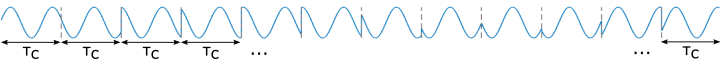
\includegraphics[width=0.9\textwidth]{simpleThermal_oneMode.png}
		\caption{\label{fig:simpleThermal_oneMode} Simple model of a single mode of thermal light: Modelled as a perfect sinusoidal wave interrupted by random phase jumps every coherence time $\tau_c$.}
		\end{figure}
	When two of these thermal modes are added together (this could represent a spontaneous emission source generating two photons at a time, or a laser with two independent modes) the waves interfere causing a different combined intensity for each $\tau_c$ period depending on the phase difference between the two modes (see fig. \ref{fig:simpleThermal_twoModes}).\\
		\begin{figure}[h]
		\centering
		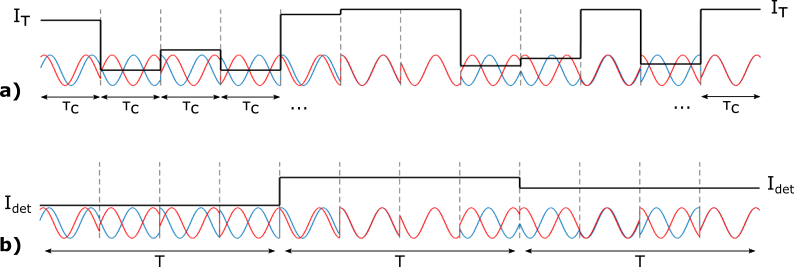
\includegraphics[width=1\textwidth]{simpleThermal_twoModes.png}
		\caption{\label{fig:simpleThermal_twoModes} Simple model of the origin and detection of PIIN: when two (or more) modes of thermal light interfere with each other, the random phase jumps will cause a random phase difference between the modes for each period $\tau_c$. \bf{a)} \normalfont The instantaneous intensity $I_{\tau}$ fluctuates strongly from one coherence period $\tau_c$ to the next, due to the modes interfering constructively or destructively depending on the instantaneous phase difference. \bf b) \normalfont When detecting for an integration time $T$ longer than the coherence time (in this case $T=4\tau_c$) the fluctuations in detected intensity $I_{det}$ weaker, as the integration averages out large fluctuations over multiple coherence times.}
		\end{figure}
	The normalised measured instantaneous intensity for each period $\tau$, given some phase difference between the two modes $\Delta \phi$, is $I_{\tau} = \frac{1+cos(\Delta \phi)}{2}$. Note that $\Delta \phi_k$ is uniformly distributed over $[0,2\pi)$. However, if the integration time of the detector $T$ is larger than the coherence time $\tau_c$ we can define the ratio $M$ as follows:
		\begin{equation}
		M = T/\tau_c.
		\end{equation}
	The normalised detected intensity thus becomes
		\begin{equation}
		I_{det} = \sum_{m=1}^M \frac{1}{M} \frac{1+cos(\Delta \phi_m)}{2}.
		\end{equation}
	Using the statistical properties of the cosine function, and the central limit theorem, we thus obtain the mean and standard deviation of the \textit{measured}, or integrated, intensity:
		\begin{equation}
		\mean{I}_{int} = \frac{1}{2}, \quad \sigma_{int} = \frac{1}{\sqrt{8M}} \propto \frac{1}{\sqrt{M}} \label{eq:simpleTwoMode_stats}.
		\end{equation}
	Importantly, what eq. \ref{eq:simpleTwoMode_stats} shows is that as the integration time $T$ gets much larger than the coherence time $\tau_c$, the ratio $M$ becomes large and the standard deviation in the detected intensity fluctuation tends to zero. This simple model therefore yields three important conclusions: Firstly, eq. \ref{eq:simpleTwoMode_stats} is consistent with our everyday experience, because for thermal light sources commonly encountered (such as incandescent lightbulbs) the coherence time is much shorter than the integration time of the human eye - and thus the PIIN is not readily observed. Secondly it indicates that to extract random numbers from PIIN the light must be measured fast, and indeed the faster it is measured the more randomness can be extracted. And thirdly, as measured noise is proportional to $1/\sqrt{M} = \sqrt{\tau_c}/\sqrt{T}$, increasing the coherence time of the thermal light source will also increase the measured noise.
	
	Even though we derived  eq. \ref{eq:simpleTwoMode_stats} for a very simple two-mode light model, the statistical properties of a fully incoherent light source are very similar (see chapter 6 in \cite{goodman_statistical_2000}). In particular, in the limit where $T>>\tau_c$, i.e. of a much longer integration time than coherence time, the measured PIIN is described by
		\begin{equation} 
		\frac{\sigma_{PIIN}}{\mean{I}_{PIIN}} = \frac{1}{\sqrt{M}} = \sqrt{\frac{\tau_c}{T}}.
		\label{eq:fullPIINstats}
		\end{equation}
	The coherence time $\tau_c$ can be approximated in terms of the light source's centre wavelength $\lambda$ and spectral width $\Delta\lambda$ as follows:
		\begin{equation}
		\tau_c = \frac{\lambda^2}{c\Delta\lambda},
		\label{eq:coherenceTime}
		\end{equation}
	where $c$ is the speed of light. By substituting $\lambda$ and $\Delta\lambda$ values for typical incoherent light sources such as LEDs or SLEDs into eq. \ref{eq:coherenceTime} we can see that $\tau_c$ will be on the sub-picosecond timescale. Integration times of photodetectors on the other hand are normally at least two orders of magnitude larger and thus we can apply \ref{eq:fullPIINstats} as we are comfortably in the $T>>\tau_c$ regime. Lastly, note that one will always measure shot noise in addition to PIIN. Further, any real set-up will also measure some technical or system noise, whose origin is not quantum in nature. We can therefore express the total detected noise in terms of PIIN, shot noise and technical noise:
		\begin{equation}
		\sigma_{total} = \sqrt{\sigma_{PIIN}^2 + \sigma_{shot}^2 + \sigma_{technical}^2}.
		\label{eq:noiseContributions}
		\end{equation}

	Now, eqs. \ref{eq:fullPIINstats} and \ref{eq:coherenceTime} show that for a given integration time a larger PIIN level can be detected for a long coherence time, which in turn requires a narrow source spectral width. The integration time $T$ on the other hand must be kept as low as possible. In past works measuring PIIN in the near-infrared from SLED sources these requirements were met by using a narrowband spectral filter on the source as well as high bandwidth photodiodes and electronics \cite{huang_real-time_2014, li_scalable_2011}.

\section{QRNG from PIIN using visible LEDs}
\subsection{Using SPAD Arrays to measure Intensity Fluctuations}
	While random number generation from PIIN has already been demonstrated for near-infrared wavelengths, this was achieved using bulky, expensive and sensitive components such as a SLED which requires careful optical isolation and precise driving current control. However, to transition to a more affordable and portable solution it would be desirable to use a simple LED light source emitting in the visible, which moreover permits the use of silicon-based photodetection. Unfortunately, as eq. \ref{eq:coherenceTime} shows, the coherence time of a light source falls quadratically as the wavelength becomes shorter, resulting in more stringent requirements on the integration time and permissible technical noise. At present, single photon avalanche diodes (SPADs) are the only detection technology for the visible wavelength range capable of achieving the low-noise readout and necessary short integration time.

	SPADs might at first glance seem a strange choice for measuring intensity fluctuations given that a SPAD is neither particularly cheap nor is it a photon number resolving device - upon detection of light a SPAD emits an electronic pulse that is identical regardless of how many photons initiated the detection event. However the recent rapid advances in SPAD arrays being fabricated using industrial CMOS processes means that both of these objections can be addressed. Firstly regarding cost, while a CMOS-fabricated SPAD array is far more expensive than regular CMOS image sensors available for cameras today, the inherent scalability of optimised CMOS processes coupled with the larger volumes being produced means that costs are already orders of magnitude lower than a few years ago, and will continue to fall \cite{abbas_cmos_2018, gyongy_$256times256$_2018, webster_high-performance_2012}. Secondly, regarding the ability to differentiate between intensities, it is true that one single SPAD only has an effective resolution of one bit. But by evenly spreading the light to be measured across the entire area of a SPAD array the intensity can be measured by the number of SPADs activated by the incoming light. SPAD arrays of size $512\times 512$ pixels have been fabricated thus far, which already gives significant intensity resolution \cite{ulku_512512_2017}.
	
	The method of detecting PIIN that we present in this report therefore needs four main components: a visible wavelength LED source, a narrowband wavelength filter, SPAD array imager, and some optics to distribute the light across the SPAD array. Remembering that according to eq. \ref{eq:noiseContributions} our set-up will measure the combination of PIIN, shot noise and technical noise, the present scheme can be seen as an extension of the method described in \cite{sanguinetti_quantum_2014}, where random numbers were generated by using a camera to measure the shot noise of an LED. Therefore the proof of principle will be provided by comparing the noise level from only shot noise and technical noise to the noise level when all three types of noise are measured. In practice, as by eq. \ref{eq:noiseContributions} only the combined total noise can be observed, to observe the PIIN contribution it is necessary to keep the shot noise and technical noise constant. This is achieved using the set-up illustrated in figure \ref{fig:ledsetup1v2}. Here light emission from an LED is detected by a SPAD array, and a removable narrowband spectral filter switches between the short coherence time (lower PIIN) and long coherence time (higher PIIN) regime. As narrowing the LED spectrum also reduces the light intensity a pair of polarisers is used as an attenuator: Rotating the polariser closest to the LED so that the measured intensities for the two coherence regimes match. This ensuring that the shot noise stays constant. As the polariser closest to the SPAD array does not change, the polarisation of the detected light stays constant which removes any dependence on detector polarisation sensitivity. And as the attenuation is a purely optical process the technical noise stemming from LED and SPAD electronics stays constant too.
		
		\begin{figure}[hb]
		\centering
		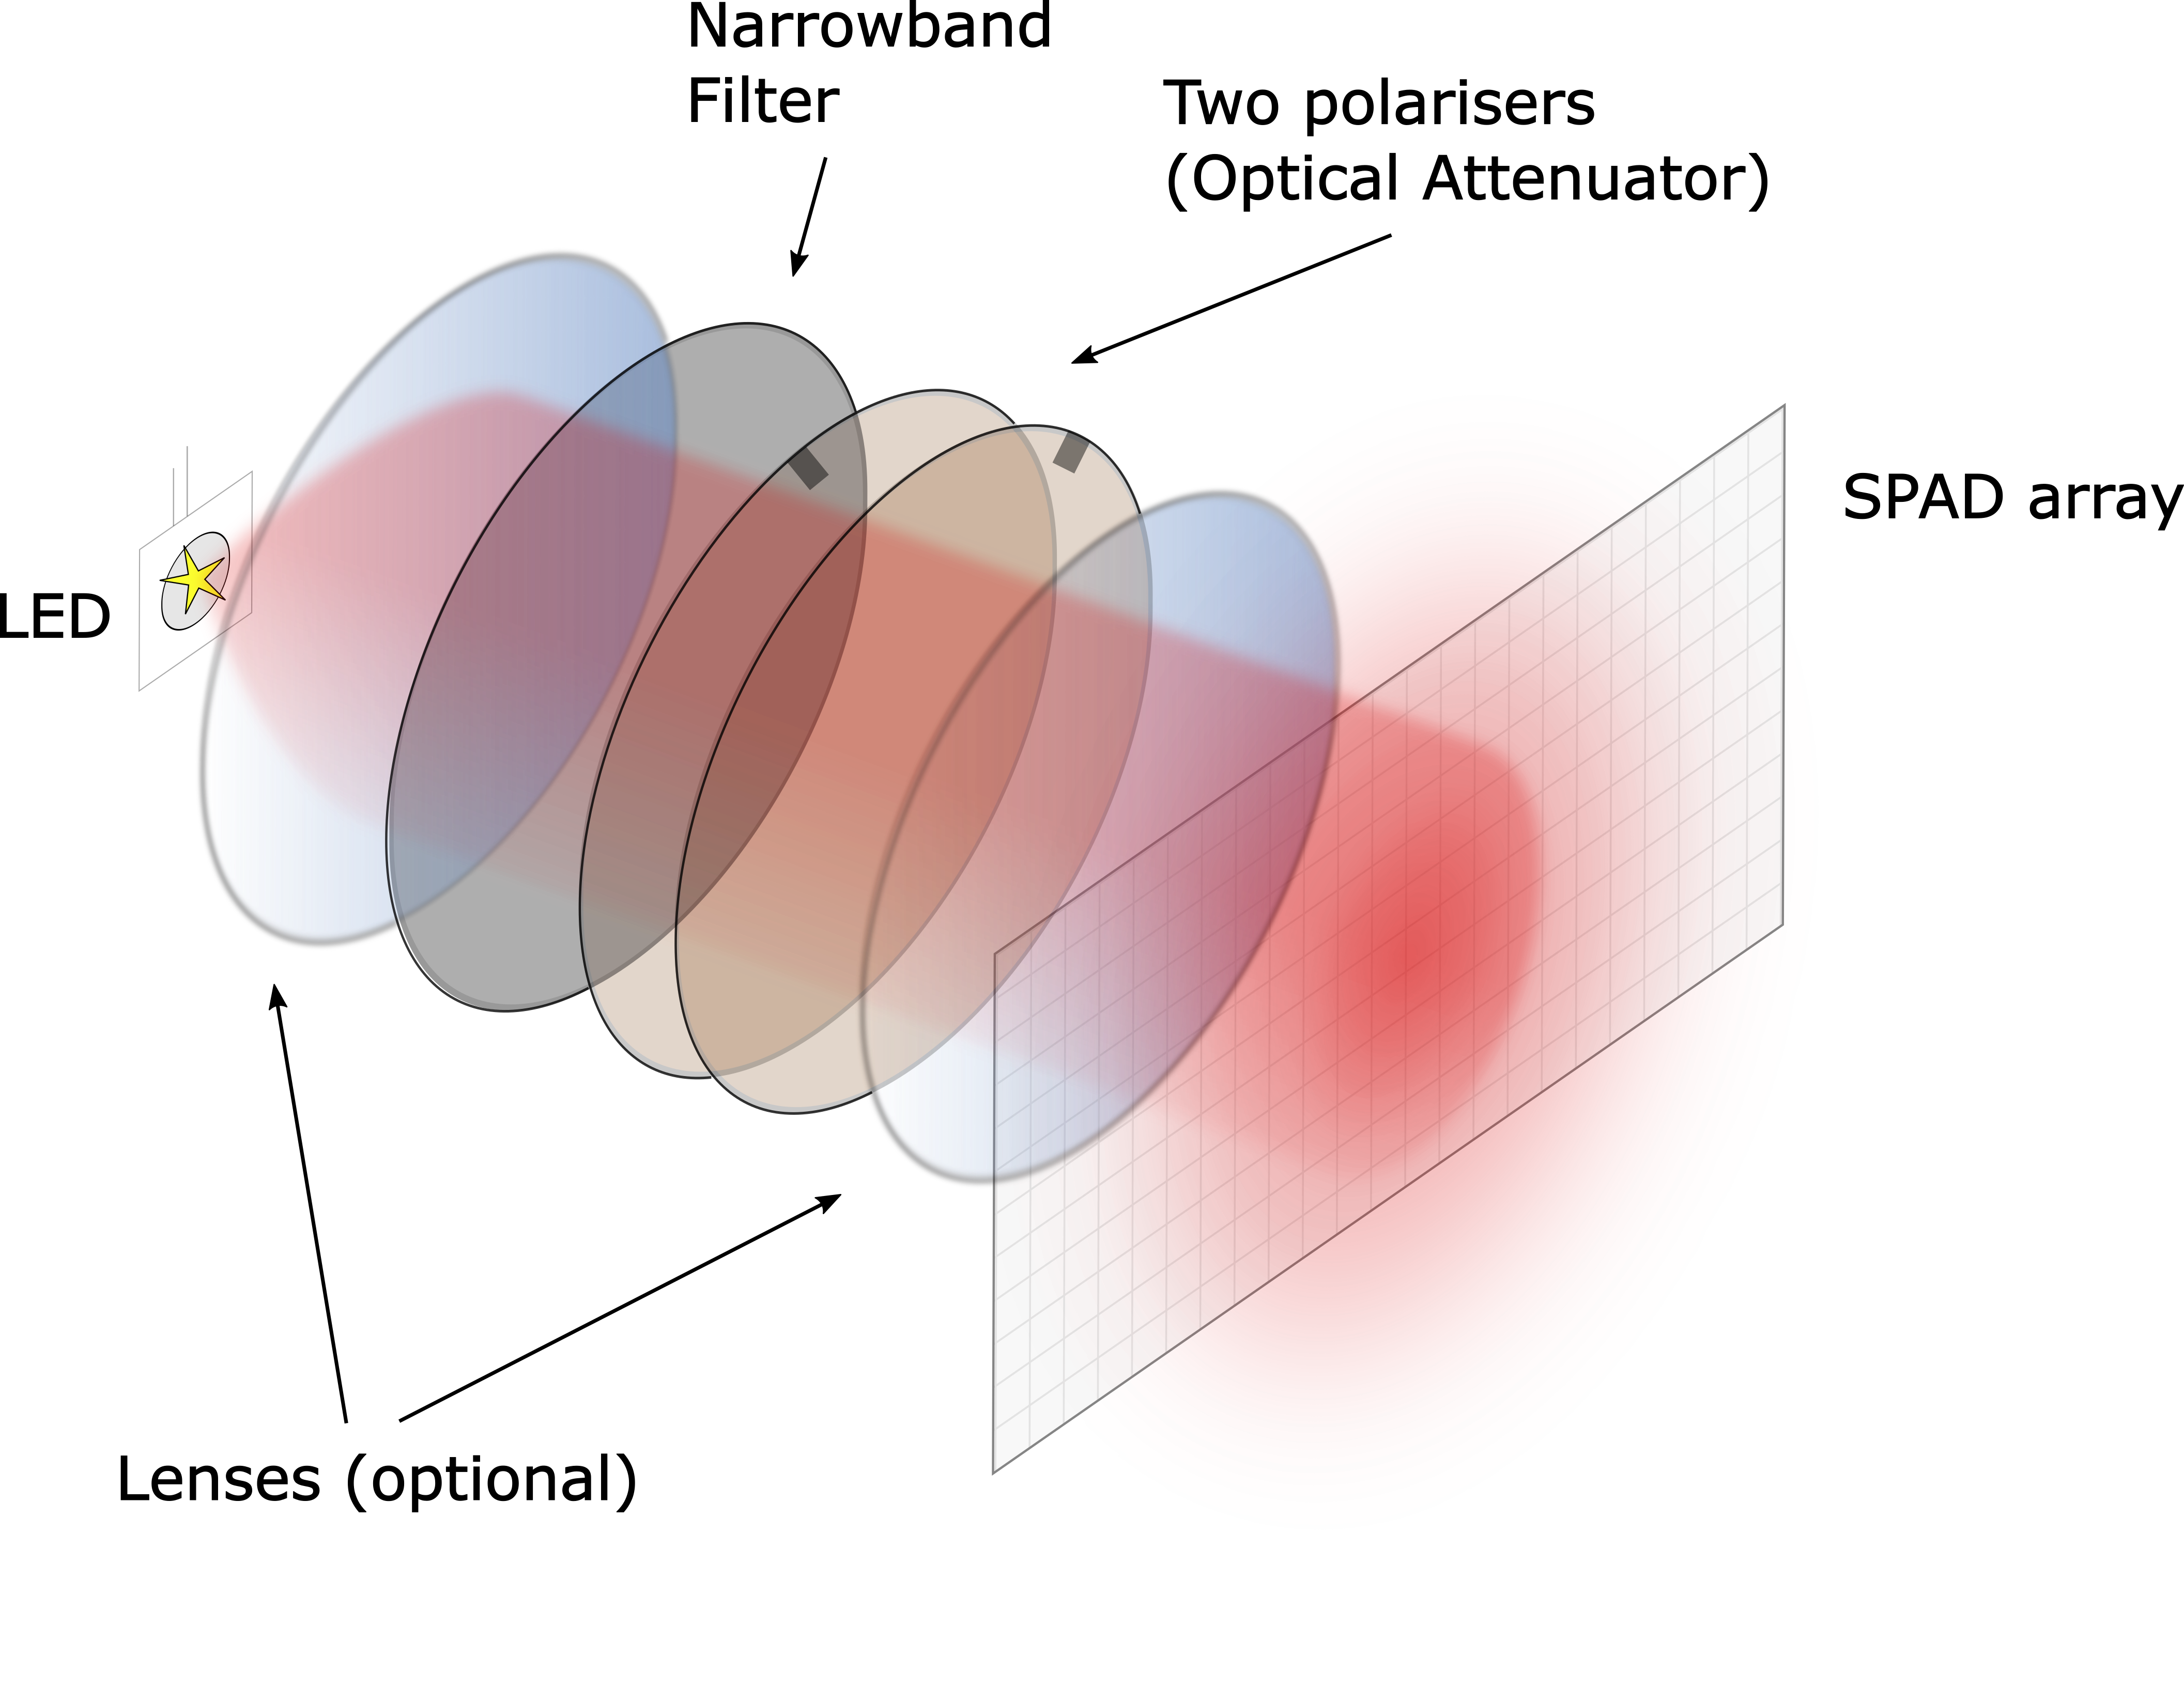
\includegraphics[width=0.6\linewidth]{Figures/LED_setup1_v2}
		\caption{Schematic of experimental set-up: The LED is collimated and optimally spread across the SPAD array using a series of lenses and/or diffusers (number and configuration of optical elements depends on etendue of LED emission and SPAD area). A removable narrowband spectral filter is used to switch between the short and long coherence time regimes and a pair of polarisers is used to optically adjust the transmitted light intensity.}
		\label{fig:ledsetup1v2}
		\end{figure}
	
\subsection{SPAD Saturation Effect}
	There is one important subtlety to take into consideration when using a SPAD array to measure intensity fluctuations: a single SPAD has a so-called dead time after detecting some light during which it is not sensitive to all subsequent photon arrivals (typically ranging from 20-100ns for silicon SPADs). That is, its saturation level is one photon per dead time, which affects the measurement of noise in the following way: Let the true light intensity incident on the sensor have some probability distribution as follows
		\begin{eqnarray}
			P(n) &=& p_n, \quad n = 0,1,2,3... \\
			\sum_{n = 0}^{\infty} p_n &=&1,
		\end{eqnarray}
	where $P(n)$ is the probability of $n$ photons arriving within one dead time period. However, within one dead time period a SPAD can only distinguish between 0 photons and 1 or more photons, and thus the detected probability distribution becomes:
		\begin{eqnarray}
			P_{det} (0) &=& p_0\\
			P_{det} (n \geq 1) &=& \sum_{n = 1}^{\infty} p_n = 1-p_0
		\end{eqnarray}
	Using the definition of variance $\sigma^2 = E(X^2) - (E(X))^2$ (where $E(X)$ represents the expected value of random variable $X$) we can calculate (or approximate) the standard deviation of the detected noise. For the case of purely Poissonian noise (shot noise), in the low $n$ regime, the true noise level and detected noise level are shown in figure \ref{fig:spadsaturationeffect}.
		\begin{figure}[h]
			\centering
			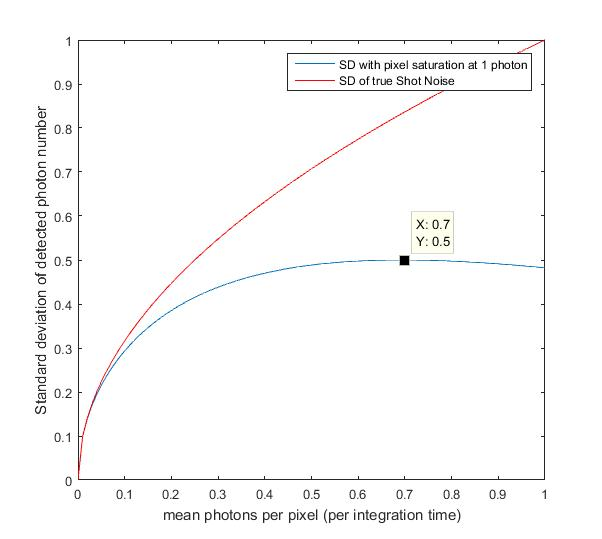
\includegraphics[width=0.5\linewidth]{Figures/SPADsaturationEffect}
			\caption{Effect of SPAD on detected Noise: For the case of pure shot (Poissonian) noise the true standard deviation is shown along with the measured standard deviation, where $n$ is the mean number of photons arriving per SPAD pixel, per dead time period.}
			\label{fig:spadsaturationeffect}
		\end{figure}
	As can be seen the detected standard deviation only accurately represents the true intensity noise level for low mean photon numbers per pixel - above around 0.3 photons per pixel the detected noise begins to saturate. In practice this means that the dynamic range per dead time of an N-pixel SPAD array is around $0.3\times N$. 
	
\section{Detection Schemes}
	For the experiments described in this report the MPD SPC3 camera was used as the SPAD array. This commercially available camera has 2048 SPAD pixels, arranged in a 64-by-32 matrix, a variable frame rate up to 96kHz and external and internal gating capabilities. All following methods are set up according to the scheme shown in figure \ref{fig:ledsetup1v2}, where a Semrock narrowband filter was used to lengthen the coherence time. As the $\tau_c$ limit is given by the narrowband filter, the primary method available to us for increasing the measurable PIIN is to decrease the integration time $T$ as much as possible. The following experimental schemes outline three methods to achieve this end.
	
\subsection{Pulsed LED}\label{scheme1}
	In the first scheme we relied on a pulsed LED illumination to provide a short effective integration time, while the SPAD array was not gated. The Picoquant PLS450 (using a PDL 800-D as the current driver) was used, which produces light pulses with a length of approximately 800ps. Fig. \ref{fig:detectionscheme1} illustrates the scheme. As the set-up is kept in the dark, light is only incident on the SPAD array when the LED emits a pulse. Source pulse rate and camera frame rate were synchronised at 62.5kHz so one light pulse arrives per camera frame and therefore the effective integration time equals the LED pulse length, as shown by the green shaded area in fig. \ref{fig:detectionscheme1} ($T = t_{LED}$). The wavelength of the source was 458nm, while the spectral width of the filter used (Semrock LL01-458-12.5) was 3nm, which by eq. \ref{eq:coherenceTime} leads to a $\tau_c$ of 0.25ps. By equation \ref{eq:fullPIINstats} the expected standard deviation due to PIIN was therefore $1.8\%$ of the intensity. In experimental trials however, no difference was observed between the low coherence and high coherence regimes, for several proposed reasons. Firstly, the detected mean intensities were on the order of 400 photons per frame, implying an expected 7-photon standard deviation due to PIIN, compared to a $\sigma_{shot} = \sqrt{400}=20$ due to shot noise, as well as technical or electronic noise. This resulted in a very low detection tolerance for distinguishing between the low and high coherence regimes in the first place. Secondly, the MPD SPC3 camera used for this trial had an extremely low fill factor - the active area of the SPAD per pixel was very much smaller than the pixel itself. This resulted in a low collection efficiency, which in turn resulted in the necessity to somewhat focus the light onto the SPAD array sensor. Due to this it is likely that the dynamic range of the detector was greatly reduced as not all pixels were receiving light, and the ones that were, were most likely saturating. The pixel fill factor will be addressed in a future upgrade to the MPD SPC3 camera with the addition of a microlens array to focus incident light onto the active area of the SPAD for every pixel.
	
	The most significant drawback of this detection scheme however was that the fast pulsed LED needs a sensitive, bulky and expensive laser diode driver (Picoquant PDL 800-D) to achieve the required pulse quality, thereby negating any advantage the SPAD detection purports to have in cost and portability in the first place. It is therefore desirable to make use of a scheme with less stringent requirements on the source electronics, and to instead use the SPAD array's gating capabilities to reduce the integration time $T$.
	
		\begin{figure}[ht]
			\centering
			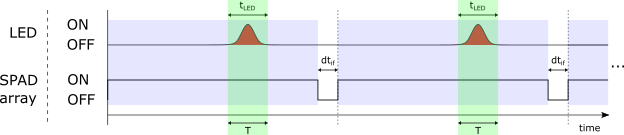
\includegraphics[width=0.8\linewidth]{Figures/detectionScheme1}
			\caption{Detection Scheme 1: Short integration time $T$ provided by pulse length of LED. The SPAD array is constantly active, only switching off for the so-called interframe dead time $dt_{if}$, which equals 10ns - at a frame rate of 62.5kHz this inactive time between frames is negligible. The LED pulse rate and SPAD array frame rate are synchronised such that one pulse arrives per frame.}
			\label{fig:detectionscheme1}
		\end{figure}
		
\subsection{Gating the SPAD array}
	The MPD SPC3 camera has extensive gating capabilities, which are worth describing in some detail at this point. Firstly, the camera has an \textit{external} gate, which is triggered through a LVTTL coaxial input (in fact, it has three external gates but we will only be using one of them). An input voltage of 0V (`0' in LVTTL logic) corresponds to the gate being open, i.e. photon counting ON. On the other hand an input voltage of 2.7V (`1' in LVTTL logic) corresponds to the gate being closed, i.e. photon counting OFF. The minimum gateable window using this external gate is 5ns. Secondly, the camera has an \textit{internal}, or software, gate which can be activated via the computer control interface. The software gate is a periodic signal, repeating every 20ns, with some configurable duty cycle: photon counting can be ON for 2ns or longer of the 20ns period with a user-configurable initial offset delay. Both the duty cycle and the initial offset can be adjusted with a (claimed) 20 ps resolution. Thirdly, both the external and the software gates can be used at the same time, in which case only those photon counts are retained for times when \textit{both} gates are on the photon counting ON setting. Also note that all gating acts globally, on all SPAD pixels at once. Lastly, all gating acts after the SPAD photodetection process. That is, the SPADs themselves are not deactivated by the gates, and detect incident photons regardless of the gate setting - the gate only determines whether a photodetection event is added to the counters and output to the connected computer or not. One important consequence of this is that if a SPAD pixel receives a photon while the gate is in the OFF setting, it will still subsequently be unable to receive another photon during its dead time even if the gate turns ON during this time. This means that when gating the SPAD detector but not the light source, the saturation condition is still determined by the dead time and not by the gate time.
	
	In order to synchronise the MPD SPC3's external gate with its frame rate it is necessary to make use of the SYNC OUT signal. The SYNC OUT signal is an LVTTL signal that is emitted by the camera's coaxial SYNC OUT output, being emitted at the start of every frame (with some constant delay due to electronic signal propagation time), having a rise time of 10ns and a pulse length of 100ns. As the SYNC OUT signal always has a constant length, but we want to be able to vary the external gate window, it is necessary to process this output pulse rather than connecting the SYNC OUT directly to the external gate IN. Moreover, we want the gate to be in the OFF setting the majority of the time, only switching on for a brief amount of time to keep the integration time $T$ as short as possible. However, as 0V corresponds to counting ON and 2.7V to counting OFF for the external gate, it is necessary to reverse the polarity of the SYNC OUT and add a constant bias voltage, such that the external gate signal is kept at 2.7V until we want to measure (and only then can it be lowered to 0V). We propose to meet these ends through the use of an FPGA receiving the camera SYNC OUT, and feeding the necessary gating voltage back into the camera. The use of an FPGA has the further advantage that it can additionally serve to synchronise a pulsed LED with the camera frame rate (see section \ref{gatedSPADandLED}). A schematic of this gating set-up can be seen in figure \ref{fig:electronics_schematic} (see caption for further description). The use of an FPGA is in addition beneficial for future cost and scalability concerns, as its function can also be performed by integrated microcircuits.
		
		\begin{figure}[h!]
			\centering
			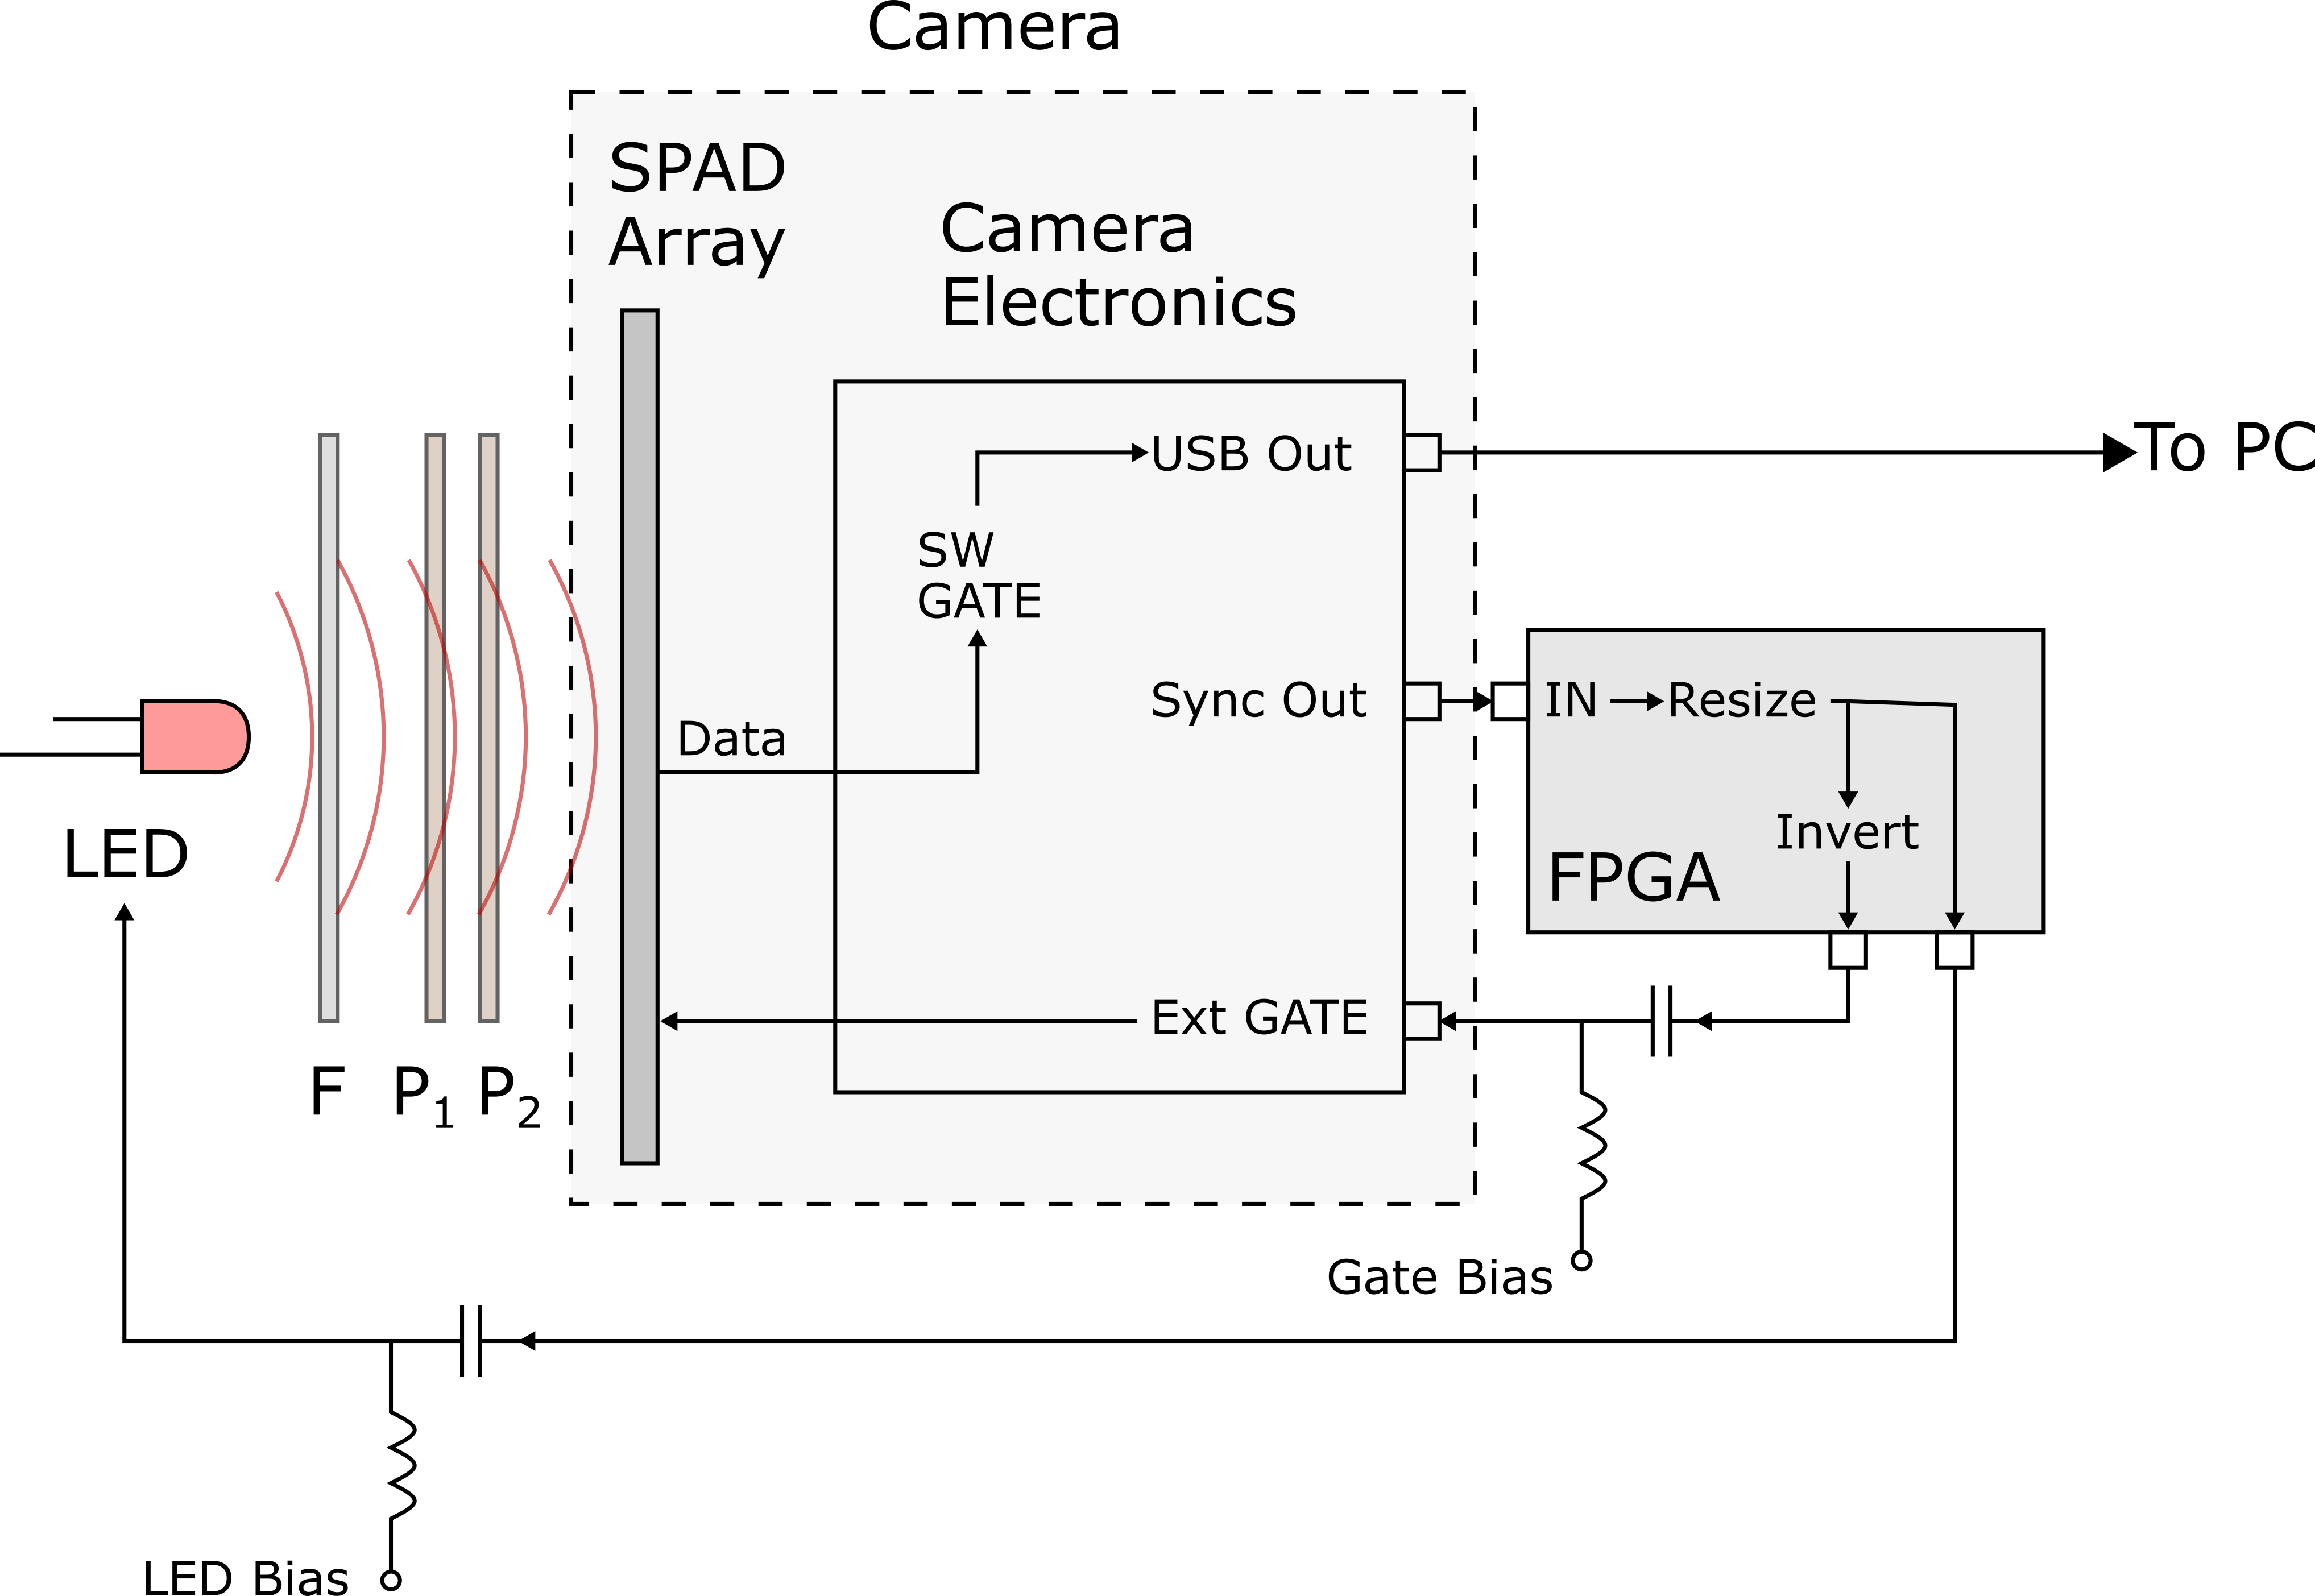
\includegraphics[width=0.8\linewidth]{Figures/electronics_schematic}
			\caption{Schematic of the electronic set-up used to gate the SPAD array, and optionally pulse the LED source: The MPD SPC3 camera sends out LVTTL signal to synchronise gating and pulsing (SYNC OUT). The SYNC OUT signal enters an FPGA, which reshapes it into a user-defined pulse length, and reverses the polarity for the camera's external gate input. DC bias voltages can be applied separately to the gate and LED signal paths. The camera receives the gate IN, which acts on the SPAD array data. The (already gated) image data is further gated by the software gate, before being transmitted to the controlling computer via USB. Also shown is the LED light source and the removable bandpass filter ($F$) and the optical attenuator, implemented with two polarisers ($P_1$ and $P_2$)}
			\label{fig:electronics_schematic}
		\end{figure}
		
	We now come to the gated detection scheme. We recall from eq. \ref{eq:fullPIINstats} that the aim is to reduce the integration time $T$. Using only the camera's external gate it is possible to reduce $T$ to 5ns, however by using both gates even lower values can be reached. This is achieved by only partially overlapping the respective ON periods for the external and software gates - the effective integration time then becomes the overlap time between the two gates. This is illustrated in fig. \ref{fig:detectionScheme2}. See the figure caption for further details of the detection scheme.
	
		\begin{figure}[h]
			\centering
			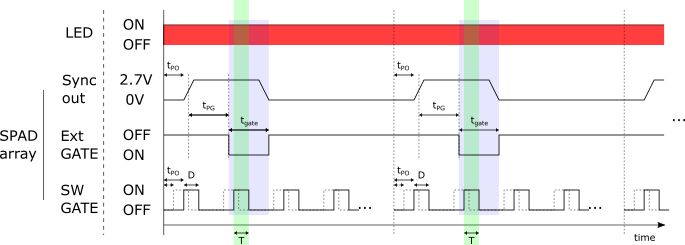
\includegraphics[width=0.7\linewidth]{Figures/detectionScheme2}
			\caption{Gated SPAD detection scheme: The SPAD array camera generates a SYNC OUT pulse some delay after the start of every frame. This pulse is reshaped and inverted by the FPGA (see fig. \ref{fig:electronics_schematic}), and after some propagation delay $t_{PG}$ triggers the external gate to the counting ON setting. The external gate stays in the ON setting for some time $T_{gate}$, discarding all photons counts from outside of this window (grey shaded box). Simultaneously the software gate is periodically switching on and then off again every 20ns, remaining ON for some user defined duty cycle time $D$, and offset from the start of the frame by some variable initial delay. Only when both gates are in the counting ON setting are the photon counts retained (green shaded area) and thus the effective integration time $T$ is given by the overlap between the two gates.}
			\label{fig:detectionScheme2}
		\end{figure}
		
	Gating the SPAD detector has the further advantage that dark counts are now practically negligible. On the other hand, without also pulsing the light source, there is one severe disadvantage: Recall that the gating does not turn off the SPADs itself, and that therefore the saturation condition is determined by the SPAD dead time and not by the gate window. For the SPC3 camera the minimum dead time is 50ns. On the other hand, due to sub-picosecond coherence times of visible LED sources, due to equation \ref{eq:fullPIINstats} the integration time should be sub-nanosecond. That is, the integration time is 50 times shorter than the saturation period! The result of this is that the dynamic range is reduced by at least a factor of 50 - in the case of the 2048-pixel MPD SPC3 this results in an unacceptably low intensity resolution. The simple solution at this point is of course to wait for the availability of larger SPAD imaging array, which will in any case increase the intensity resolution. However by gating the detector as well as pulsing the source, sufficient intensity resolution can be obtained with smaller SPAD arrays.
	
\subsection{Gating the SPAD array and pulsing the LED} \label{gatedSPADandLED}

	As shown in fig. \ref{fig:electronics_schematic}, a FPGA to process the camera SYNC OUT signal can also be used to pulse the LED. Now, by synchronising the LED such that it only turns on once the camera gate is already in the ON setting we can ensure that all pixels were in the dark prior to this and thus are not in the inactive, dead time period when the gate opens. This is illustrated schematically in fig. \ref{fig:detectionScheme3b}. As can be seen, it is important that the respective propagation delays from the camera SYNC OUT to the external gate and to the LED are carefully matched. In particular, the camera gate must turn ON before the LED emits, however the LED must also have turned on before the camera gate turns OFF again. While this is doubtless one experimental difficulty, this method is nonetheless more practical and less costly than the one described in section \ref{scheme1}. This is because there are no stringent requirements on the length of the LED pulse, as long as it is significantly shorter than the frame time, thereby foregoing the need for high speed driving electronics.
	
		\begin{figure}
			\centering
			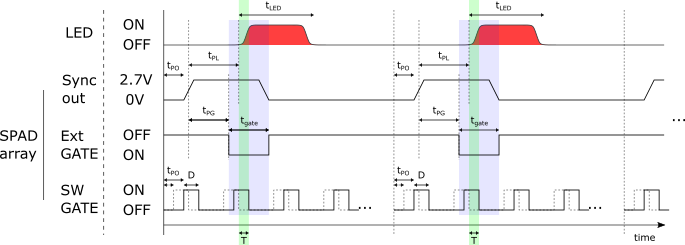
\includegraphics[width=0.7\linewidth]{Figures/detectionScheme3b}
			\caption{Gated SPAD with pulsed LED: Detection scheme as in fig. \ref{fig:detectionScheme2}, but with the SYNC OUT also being used to trigger LED emission. After a SYNC OUT pulse is emitted from the camera, after propagation delay to the LED $t_{PL}$, the LED illuminates. As long as $t_{PG}<t_{PL}<t_{PG}+t_{gate}$, the effective integration time $T$ is given by the overlap between the two gates and the LED pulse (green shaded area).}
			\label{fig:detectionScheme3b}
		\end{figure}

\section{Future Improvements}
	
	The most important contribution to future improvement of the QRNG method outlined in this report will doubtless simply be the availability of SPAD arrays with more pixels at a continually lowering price. In addition, next-generation SPAD arrays will have the ability to time-tag individual photon detections on each pixel \cite{antolovic_spad_2017}. This will allow the post-selection of effective integration times on the order of tens of picoseconds. Secondly, fast LED pulse times thus far require expensive and bulky current driving electronics. However, there has been recent progress in using plasmonics to decrease the rise time for LEDs, and to lower the requirements on driving electronics \cite{tsakmakidis_large_2016}. This could result in an improvement of the method described in section \ref{gatedSPADandLED}, or even render the method from section \ref{scheme1} viable. Thirdly, while technically more demanding, there has been progress in implementing effective sensor-level gating. That is, in gating SPADs such that the detector does not register the incidence of an incoming photon (with the associated following dead time) while the gate is set to counting OFF \cite{tosi_fast-gated_2011}. Implementing sensor-level gating would negate the need to pulse the source, as the sensor saturation condition would now indeed be given by the gate window. Lastly, from a more immediate practical perspective, the next development will be to miniaturise the entire set-up and increase optical efficiency. The latter goal can be achieved by making the light source an array of LEDs rather than a single LED. Passing the light through a diffuser onto the SPAD array should result in an even sensor illumination and thus the utilisation of the full available dynamic range.
	
\clearpage
\bibliographystyle{ieeetr}
\bibliography{cameraQRNG_bib}

\end{document}